
\documentclass[review,authoryear]{elsarticle}
% \documentclass[3p,authoryear,twocolumn]{elsarticle} %Just to give a feel of how it would look like

\usepackage[utf8]{inputenc}
\usepackage{xcolor}
\usepackage{amsmath}

\newcommand{\memo}[2]{\textcolor{#1}{#2}}
\newcommand{\xavi}[1]{\memo{orange}{xavi: #1\\}}
\newcommand{\enrico}[1]{\memo{blue}{enrico: #1\\}}

\journal{Theoretical Population Biology}

\begin{document}

\begin{frontmatter}

\title{Allee Effect and Cultural Evolution}
%\title{The evolution of payoff-biased learning under Allee Effect} %Perhaps a 


\author[label1,label2]{Enrico R. Crema\corref{cor1}}
\cortext[cor1]{Corresponding Author: enrico.crema@upf.edu}
\author[label3]{Xavier Rubio-Campillo}

\address[label1]{CaSEs - Complexity and Socio-Ecological Dynamics Research Group, Barcelona}
\address[label2]{UCL Institute of Archaeology}
\address[label3]{BSC - Barcelona Supercomputing Center}



\begin{abstract}
Several social learning strategies are guided by an evaluation of alternative cultural variants by means of the expected payoffs associated by these. The assumption of the social learner is that the payoff received by the transmitter while expressing a given cultural trait, is a proxy for for inferring the qualitative features of the trait itself. Here we explore the theoretical implications when payoff directly affects reproductive fitness and it is density dependent, that is its expected amount is a function of the number of individuals possessing the same trait. More specifically we consider situations where the density dependence is simultaneously direct and inverse, whereby the highest payoff is achieved at intermediate densities. This non-linear relationship, known as Allee effect, portrays a large number of behavioural traits that are enhanced by cooperation or mutual facilitation, but are somehow constrained by some carrying capacity.  We  explores the evolutionary dynamics of a single trait model with two variants, each exhibiting a different Allee effect. We used a modified Lotka-Volterra model of payoff-biased social learning, and show that different degrees of reliance on social learning can exhibit a variety of equilibria, including episodes of reversion, stable co-existence, and fixation to single variant.

\end{abstract}

\begin{keyword}
Social Learning\sep Subsistence\sep Allee Effect\sep Cooperation\sep Carrying Capacity
\end{keyword}

\end{frontmatter}

\section{Introduction}

The last three decades have witnessed a steady growth of formal models of cultural evolution. Early works inspired by population biology \citep{cavallisforza_feldman_1981,boyd1985} have laid the foundation of a now mature trans-disciplinary field which unites the social and biological sciences \citep{mesoudi_etal_2006}. The rich cross-fertilisation between different fields has fomented the designing of new analytical techniques as well as new usage for existing methods, but more crucially have prompted the development of theoretical models of how culture is acquired and transmitted between individuals~\citep{mesoudi_cultural_2015}.

A central element, shared by most models of social learning, is the existence of some heuristics that promotes the selection of a given cultural variant over another \citep{laland2004}. This can be based on some properties of the variant itself (\emph{content bias}) or derived from contextual cues (\emph{context bias}), such as the commonness or the rareness of a trait (\emph{conformist bias} and \emph{anti-conformist bias}), or some features associated with the transmitter such as prestige, success, or similarity to the learner (\emph{context bias})\citep{henrich_mcelreath2003}. 

This paper examines a group of social learning strategies generally referred to as \emph{payoff-based transmission} \citep{schlag1998,kendal_etal_2009,lake_and_crema_2012,baldini2013,kandler_and_laland_2013,crema_lake_inpress}. Here the probability of copying a cultural variant $i$ is directly proportional to a payoff $s$ observed amongst individuals possessing $i$. In other words the social learner assumes that the success of an individual (measured in $s$) is to some extent function of the observed behavioural trait, that is $s=f(i)$. Several variants of this learning strategies have been proposed and explored, including: \emph{imitate the best}, where the social learner identifies and copies the trait possessed by the individual with the highest payoff; \emph{compare means}, where the social learner compare the average payoff of different strategies and chooses the highest variant; and the \emph{proportional imitation rule}, where the probability of adopting a variant is proportional to the difference in payoff between the demonstrator and the learner~\citep{schlag1998,baldini2013}. 

Whilst most studies focused on how difference in these imitation rules can drive the dynamics of the system, less attention has been given to the relationship between target cultural traits and their payoff signals. Typical signal are most likely some indirect proxy of success (e.g. number of offspring, income, presence/absence of other traits associated with success or prestige, etc.)  that are assumed, by the social learner, to be more or less linked with a cultural trait. In most cases the causal link between the payoff and a cultural trait is just inferred, and the exact processes and variables leading the latter to the former is most likely unknown. This implies that the strength of correlation between payoff and cultural trait can vary, introducing different degrees of uncertainty that can have a strong impact to the efficiency of specific learning rules. For example,~\citet{crema_lake_inpress} have shown that \emph{imitate the best} is becomes increasingly detrimental with high payoff uncertainty and a large pool of potential social teachers. This is because innovations are by definition rare in a population, and hence even if their average payoff are higher than extant suboptimal alternatives, their probability of signalling the highest payoff, and hence be selected, is low.

This uncertainty in the payoff signal is derived by the presence of interacting cultural and physical traits, as well as the environment where the trait is manifest. Thus the function $s=f(i)$ should be better described as $s=f(i,\epsilon)$, where $\epsilon$ represent all additional hidden and latent variables that contributes, along with the cultural variant of interest $i$, to the payoff signal $s$. A trivial example is a fisherman who might evaluate the performance of a new hook (the target cultural trait) using as a cue the number of fish captured (the payoff signal). The correlation between the two is partly derived by the efficiency of the hook, but also by the rod, the choice of the bait, the availability of the prey species, the choice of the fishing spot, the physical strength of the fisherman, and chance. In many cases we should expect that the social teacher and learner share many of these interacting traits as well as the environment where these are displayed. In other words, cultural and ecological inheritance should in part reduce the impact played by $\epsilon$, and consequently the uncertainty in the payoff-signal. There are however exceptions. One of these are contexts where the success of a variant is strongly correlated with the absolute number of individuals $n_i$ possessing the same trait ($i$) within a population. This density dependence, which can be described by the payoff function $f(i,n_i)$, implies that the adoption (or abandonment) of a trait can alter its expected payoff-signal, possibly generating a variety of feedback mechanism.  

Several behavioural traits are expected to show such density dependence. In particular, behaviour linked to the exploitation of limited resources are expected to exhibit density dependence. Novel optimal variants are likely to spread rapidly when the trait is rare, but once a threshold frequency is exceeded (i.e. the carrying capacity),  beneficial effect will start to decline, the payoff will become smaller, and eventually rarer suboptimal variants can be preferred (see Lake and Crema \citeyear{lake_and_crema_2012} for an extensive analysis). 

However, density dependence does not necessarily imply only a negative correlation between population size and payoff. In many ecological contexts per capita growth rate is positively correlated with population density, thus resulting into an inverse density dependence. This phenomena, known as \emph{Allee} effect \citep{allee1958,courchamp_etal_1999}, is generally explained by a range of processes including cooperation, mutual facilitation, and environmental conditioning; all processes that we expect to observe  in many cultural traits. The Allee effect has been extensively studied  from  empirical and theoretical standpoints, and its implications assessed for a variety of phenomena, including habitat selection \citep{greene_and_stamps_2001}, resource competition \citep{jang2013},  dispersal \citep{steele_2009}, shifts in settlement pattern \citep{crema_2014}, colonisation events,  \citep{kennet_etal_2006}, genetic diversity \citep{roques_etal_2012} and extinction of languages \citep{sutherland_2003} . Yet, despite this wide array of applications, we are unaware of any theoretical studies exploring how the simultaneous presence of direct and inverse density dependence in the payoff signal can affect the evolutionary dynamics of cultural transmission.   

Although a systematic review and a shared theoretical framework akin to those proposed in population ecology \citep{kramer_etal_2009} is not present in the social sciences, there are several lines of evidence supporting the existence of both direct and inverse density dependence in cultural and behavioural traits. For example several ethnographic studies on small scale societies show how the per-capita return of hunting groups show higher yield when the group size is not too small nor too big~\citep{hill_and_hawkes_1983,janssen_and_hill_2014}. Other instances of inverse density dependence include population level activities such as the use of anthropogenic fire~\citep{bird2013} or selective hunting~\citep{dods_2002} which often require a population size above a certain critical density in order to promote sufficient niche enhancement and a consequent increase in payoff~\citep{rowley-conwy_and_layton_2011}. In a broader sense any cultural trait that benefits from direct or indirect cooperation, 
%Add reference \citep{}
promote positive niche construction \citep{vandermeer_2008}, and requires a critical mass \citep{rogers_2003} are likely to exhibit some degree of Allee effect. This is thus not limited necessarily to the domain of traits directly promoting reproductive fitness, and hence can include language~\citep{kandler2009}, organisational populations~\citep{caroll_and_hannan_1989} and communication technologies \citep{van_slyke_perceived_2007}.

Here we explore the consequences of Allee effect in the evolutionary dynamics of cultural transmission, assuming that: 1) the social learning strategy is payoff-based; and 2)  the payoff is equivalent to the reproductive fitness of each individual. We will demonstrate, by means of a difference equation, that direct and inverse density dependence can strongly affect the evolutionary trajectory of the system, leading to changes in the conditions required to reach specific equilibria, as well as to the emergence of unstable patterns characterised by temporary or permanent episodes of shifts between alternative cultural variants.

\section{The Model}
We consider the evolutionary dynamics of two mutually exclusive cultural variants which payoff functions are characterised by an Allee effect. We assume a non-fixed population of size $N$, subdivided into two subpopulations with sizes $a$ and $b$, each associated with the two cultural variants. We further assume that $a$ and $b$ can change as a result of intrinsic population growth/decline as well as shifts from one to the other as a result of cultural transmission. The core model can be depicted with the following coupled difference equation \eqref{eq1}:

\begin{equation}
\begin{aligned}
a_{t+1}& = a_t + a_t R_{a,t} + C_{a,b,t} \\
b_{t+1}& = b_t + b_t R_{b,t} + C_{a,b,t}
\label{eq1}
\end{aligned}
\end{equation}

where $a_{t+1}$ and $b_{t+1}$ are the population sizes of each variant at time $t+1$. This is given by the number of individuals during the previous time-step ($a_t$ and $b_t$), the reproductive rate of each population ($R_{a,t}$ and $R_{b,t}$), and the shift from one population to another as a result of cultural transmission ($C_{a,b,t}$).

The reproductive growth rate $R$ of each population is defined by the following set of equations:

\begin{equation}
\begin{aligned}
R_{a,t}& = r_a (\frac{a_t}{A_a}-1)(1-\frac{a_t}{K_a})\\
R_{b,t}& = r_b (\frac{b_t}{A_b}-1)(1-\frac{b_t}{K_b}) 
\label{eq2}
\end{aligned}
\end{equation}

where $r$ is the basic growth rate, $A$ is the critical density and $K$ is the carrying capacity, following the condition $0<A < K$. 

Equation \eqref{eq2} depicts the so called \emph{strong} Allee effect \citep{Wang_and_Kot_2001}, where the reproductive rate is negative when population density is either below $A$ or above $K$, and  in this case reach its maxima $R_{max}=\frac{r(A-K)^2}{4AK}$ when density is equal to $\frac{(K-A)}{2}$. 

The cultural transmission component of equation \eqref{eq1} is based on the \emph{proportional imitation rule} \citep{schlag1998}. In this case, the probability of an individual with lower growth rate to adopt the trait of an individual with higher growth rate is proportional to the difference in the growth rates. This is formally portrayed as follows:

\begin{equation}
\begin{aligned}
\label{eq3}
C_{a,b,t} = 
\begin{cases}
0& \text{if } R_{a,t} = R_{b,t}\\
\zeta(a_t+a_tR_{a,t})& \text{if } R_{a,t} > R_{b,t}\\
-\zeta(b_t+b_tR_{b,t})& \text{if } R_{a,t} < R_{b,t}
\end{cases}
\end{aligned}
\end{equation}

where $\zeta$ defines the proportion of individuals changing strategy, and given by \eqref{eq4}:

\begin{equation}
\begin{aligned}
\label{eq4}
\zeta = 
\begin{cases}
z& \text{if }|R_{a,t}-R_{b,t}| > m\Delta\\
z\frac{|R_{a,t}-R{b,t}|}{m\Delta}& \text{if }|R_{a,t}-R_{b,t}| \leq m\Delta\\
\end{cases}
\end{aligned}
\end{equation}

where $z$ is a measure of reliance in social learning (effectively equivalent to highest possible transmission rate), $\Delta$ is the maximum between $R_{max(a,t)}$ and $R_{max(b,t)}$, and $m$ is a calibration parameter that measures the perception of the difference in the payoffs (i.e. small values of $m$ determines a higher rate by which the theoretical maximum transmission rate is reached). 

\section{Results}


%I attached the list of results that I sent you over the email that we need  to put in the text

%1)With no Allee effect the strategy with the highest payoff wins  /// This is obvious we don?t need to prove this 
%2) With carrying capacity, but no Allee effect we get possible cases of reversions. //Lake and Crema explores this, but the model has also uncertainty in the payoff signal so not sure if it is technically comparable? Should we do something with this?
%
%
%** Expected pattern without transmission **
%-3)We have our unstable nodes, stable nodes, and extinction. As long as the strategies are above their critical densities, they will survive. // DONE
%
%** Expected pattern with transmission **
%4) There is a possibility for a trait to not get extinct even if its below its critical density. This happens only if: a) the alternative strategy is also below the critical density and its distance from A is further b) the alternative strategy is beyond carrying capacity. If the alternative strategy is in the positive payoff interval the focal strategy will go extinct /// This is shown with all the basin plots,  so no need to anything extra.
%
%5) If both traits are above their respective critical densities, we expect stable coexistence when there is no transmission, but when z>0, strategies that are closer to their critical densities have a non-zero probability to go extinct. This probability increases as the alternative population approaches its own K or A. /// This is shown by the basin plots, so its fine.
%
%6) As a corollary to point 5, with increasing z (but also as a function of lambda), the shared perimeter of the boundary of the basin of attractions of the two strategies increases in proximity to the both critical densities. This means that small changes in behaviour (z) or external fluctuations can promote the adoption of one or the other but not the both. // This is hard to prove I guess, and not sure if the basin plots are sufficient to state this.
%
%7) If both variants have initial conditions within their positive payoff density ranges, a decrease in lambda promotes the coexistence of both strategy for a given value of z. Thus with increasing ?distance? between the two strategies, its less likely that we observe the dominance of one or the other. We ought to find out why this is the case though, perhaps we need to look at individual time-series to have some clues. // We should be able to see this with the overlap analysis + possibly individual time-series to get some grips
%
%8) With increasing values of z, the basin of coexistence is decreased to the expense of limit cycles (can we check if it is non-chaotic using Lyapunov?) and extinction of one strategy or the other. The growth is however asymmetric (maybe), and the strategy with high A and K have will have a smaller proportion of initial conditions where it can dominate. // overlap analysis should, hopefully, still show this.
%
%9) If point 8 is true, we can then argue that transition to strategies with higher carrying capacity is difficult, and entails in many case stable or unstable forms of coexistence. The only exception is when the two strategies is interacting //competition analysis, with competition values and two transmission settings.
%
%10) or the critical densities are the same // just a single basin plot would suffice. 




We investigate the equilibrium conditions for different initial population sizes of $a$ and $b$ and different settings of $z$, $A$, and $K$, ensuring that in all cases $K_b \geq K_a$. We assumed that two strategies differed only in their critical densities and carrying capacities but not on their intrinsic payoffs. To achieve this we set $r_b=\rho r_a$, where $\rho$ is a constant\footnote{Given two variants with the same baseline growth rate (i.e. $r_a=r_b$), equation \eqref{eq2} result into a lower $R$ for the variant with higher $A$ and $K$. In order to avoid this we increased the baseline of the strategy with lower $R$ by a factor $\rho$, given by the following equation:
\begin{align*}
\rho=\frac{A_bK_b(K_a-A_a)^2}{A_aK_a(A_b-K_b)^2}
\end{align*}
  } 
that ensures that the two variants have always the same $R_{max}$. Given that equations \ref{eq1}-\ref{eq4} have no analytical solution, we identified equilibrium conditions via simulation (source codes of the simulation can be found on the following repository \textcolor{red}{PUT LINK HERE})

\subsection{Equilibrium conditions without social learning}

When $z=0$, equations \ref{eq1}-\ref{eq4} becomes a standard cubic growth model with Allee effect, where the success (or failure) of a given focal trait is exclusively given by its own density. For a generic cultural trait $x$, the model predicts three equilibrium points at $x=0$ (extinction), $x=A_x$, and $x=K_x$. The equilibrium $x=A_x$ is unstable for all values of $r_x$, whereas the stability of the node at $x=K_x$ is a function of the per capita growth rate $r_x$. Increasing the latter decreases the stability of fixed points~\citep{scheuring_1999}, leading to the transition from point attractors (with equilibrium at $x=K_x$), to limit cycles and chaotic dynamics with islands of stability (see fig. \ref{fig:bifurcationDiagram}). 

\begin{figure}[h!]
  \centering
      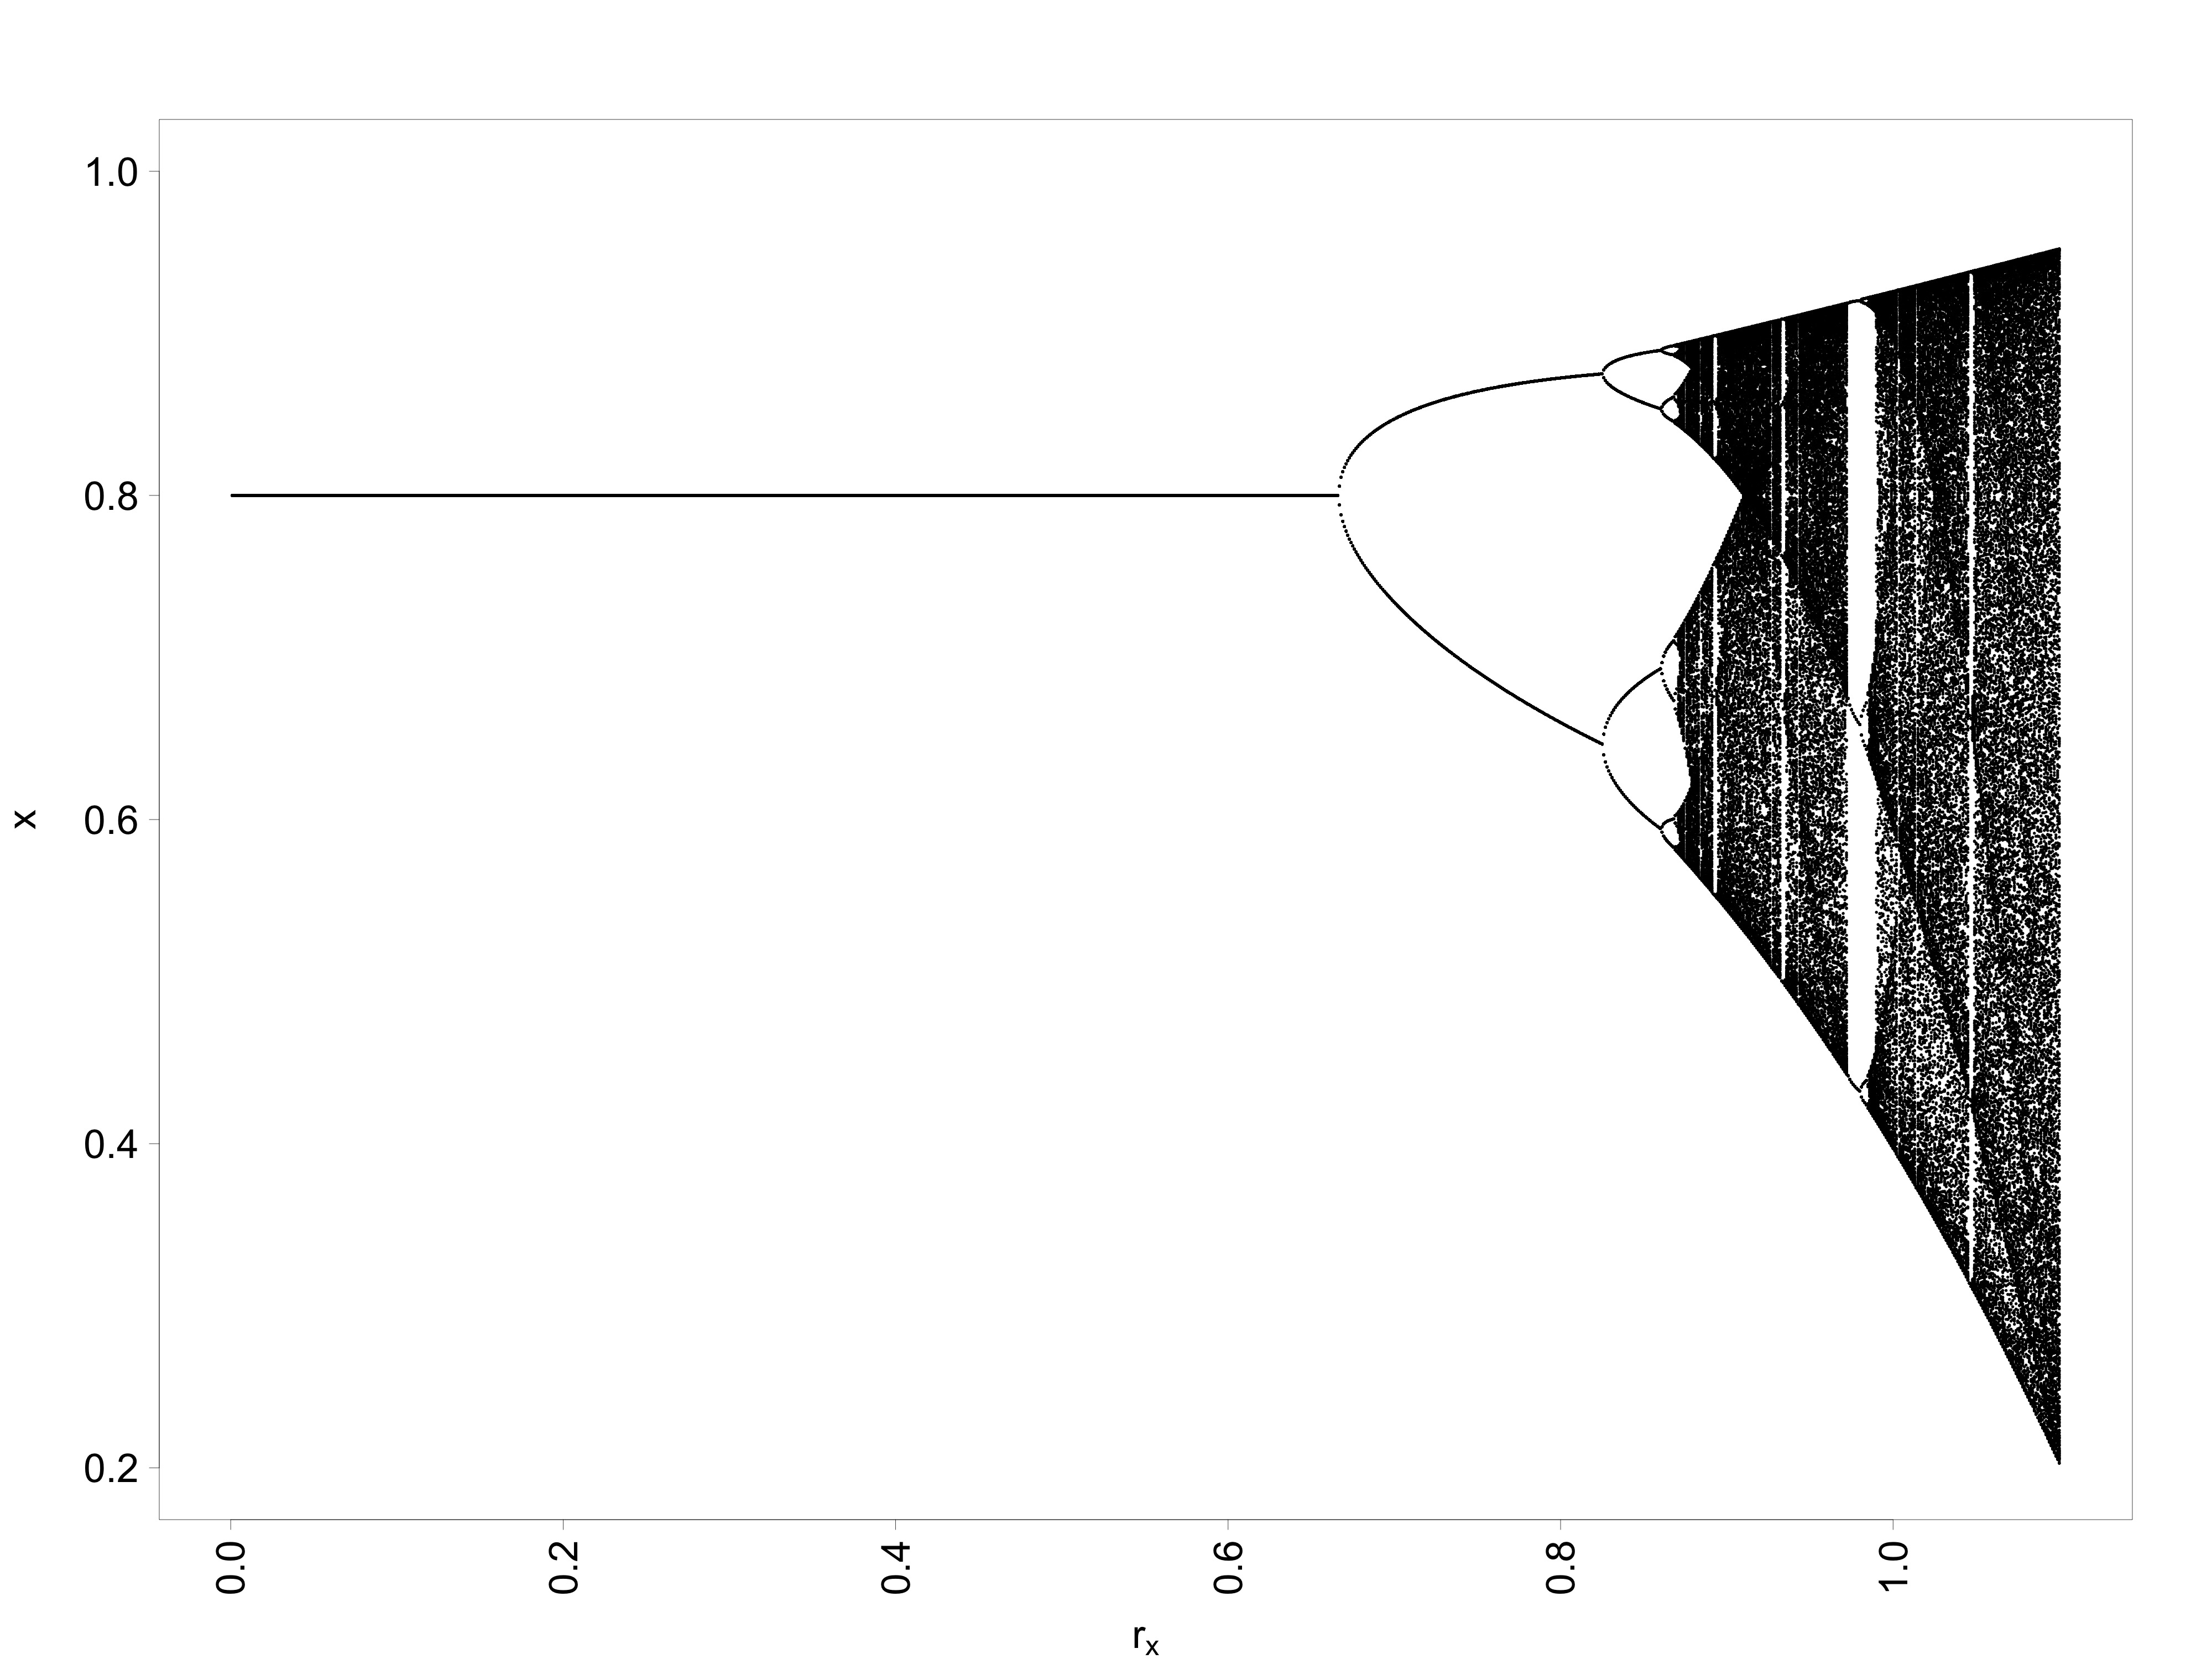
\includegraphics[width=1\textwidth]{./figures/figure1.jpg}
  \caption{Bifurcation diagram of a single population model with $A_x=0.2$ and $K_x=0.8$. For $0<r_x<0.6649747$, any initial value of $x$ greater than $A_x$ converges to $K_x$.}
    \label{fig:bifurcationDiagram}
\end{figure}

For the rest of the paper we will consider only scenarios where the node $x=K_x$ is stable. In this case the initial value of $x(t=0)$ will determine the ultimate equilibria of the system: extinction, if $x(t=0)<A_x$; unstable equilibrium, if $x(t=0)=A_x$; and stable equilibrium, if $x(t=0)>A_x$. Thus in a 2-trait model, the coexistence of both variants is guaranteed only when the initial density of both traits are above their respective critical densities, otherwise we should expect that either (i.e. $a(t=0) \geq A_a$ and $b(t=0)<A_b$ or $a(t=0)<A_a$ and $b(t=0) \geq A_b$) or both (i.e. when $a(t=0)<A_a$ and $b(t=0)<A_b$) variants are ultimately extinct (see fig. \ref{fig:NoTransmissionBasin}). 

\begin{figure}[h!]
  \centering
      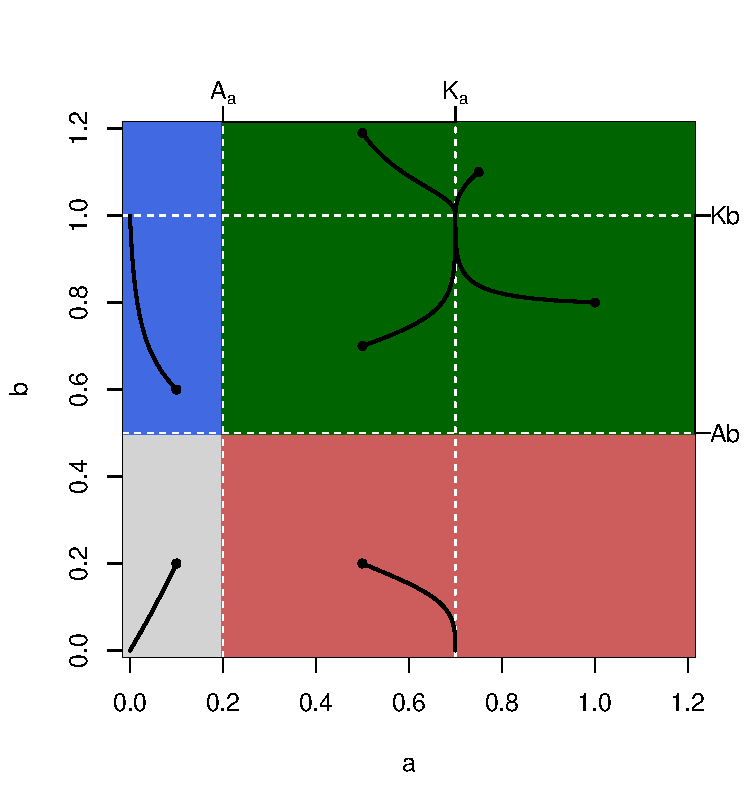
\includegraphics[width=1\textwidth]{./figures/figure2.pdf}
  \caption{Basins of attraction for the four equilibria (mutual extinction: grey; extinction of $a$: blue; extinction of $b$: red; stable coexistence: green). Solid lines represent trajectories of the system for different initial conditions, represented by dots. Model parameters: $A_a=0.2$; $K_a=0.7$; $A_b=0.5$; $K_b=1.0$; $r_a=r_b=0.05$}.
    \label{fig:NoTransmissionBasin}
\end{figure}

\subsection{Effects of social learning}

When social learning is enabled (i.e. when $z>0$), the stability of the nodes are perturbed by individuals switching from one strategy to another. We identify two major changes in the equilibrium properties of the system as a result of cultural transmission. 

First, the shape of the basins of attraction are altered, and hence initial conditions closer to the boundaries between one basin and another will be strongly affected,  leading occasionally to very different evolutionary equilibria. Figure \ref{fig:TransmissionBasin} shows an example of this. When social learning is not present (fig.~\ref{fig:TransmissionBasin}a), the initial conditions $i$, $j$, and $k$ result into a stable equilibrium at $a=K_a$ and $b=K_b$, whilst the starting point $l$ leads to the extinction of $b$. When $z=0.05$ (fig.~\ref{fig:TransmissionBasin}b), the basins of attractions are modified, resulting into different trajectories and in some cases different equilibria for the same initial conditions. Thus $i$ and $k$ are no longer leading to the coexistence of both traits but to the demise of one or the other, whilst $l$ now ensures the coexistence of both variants. 

\begin{figure*}
  \centering
      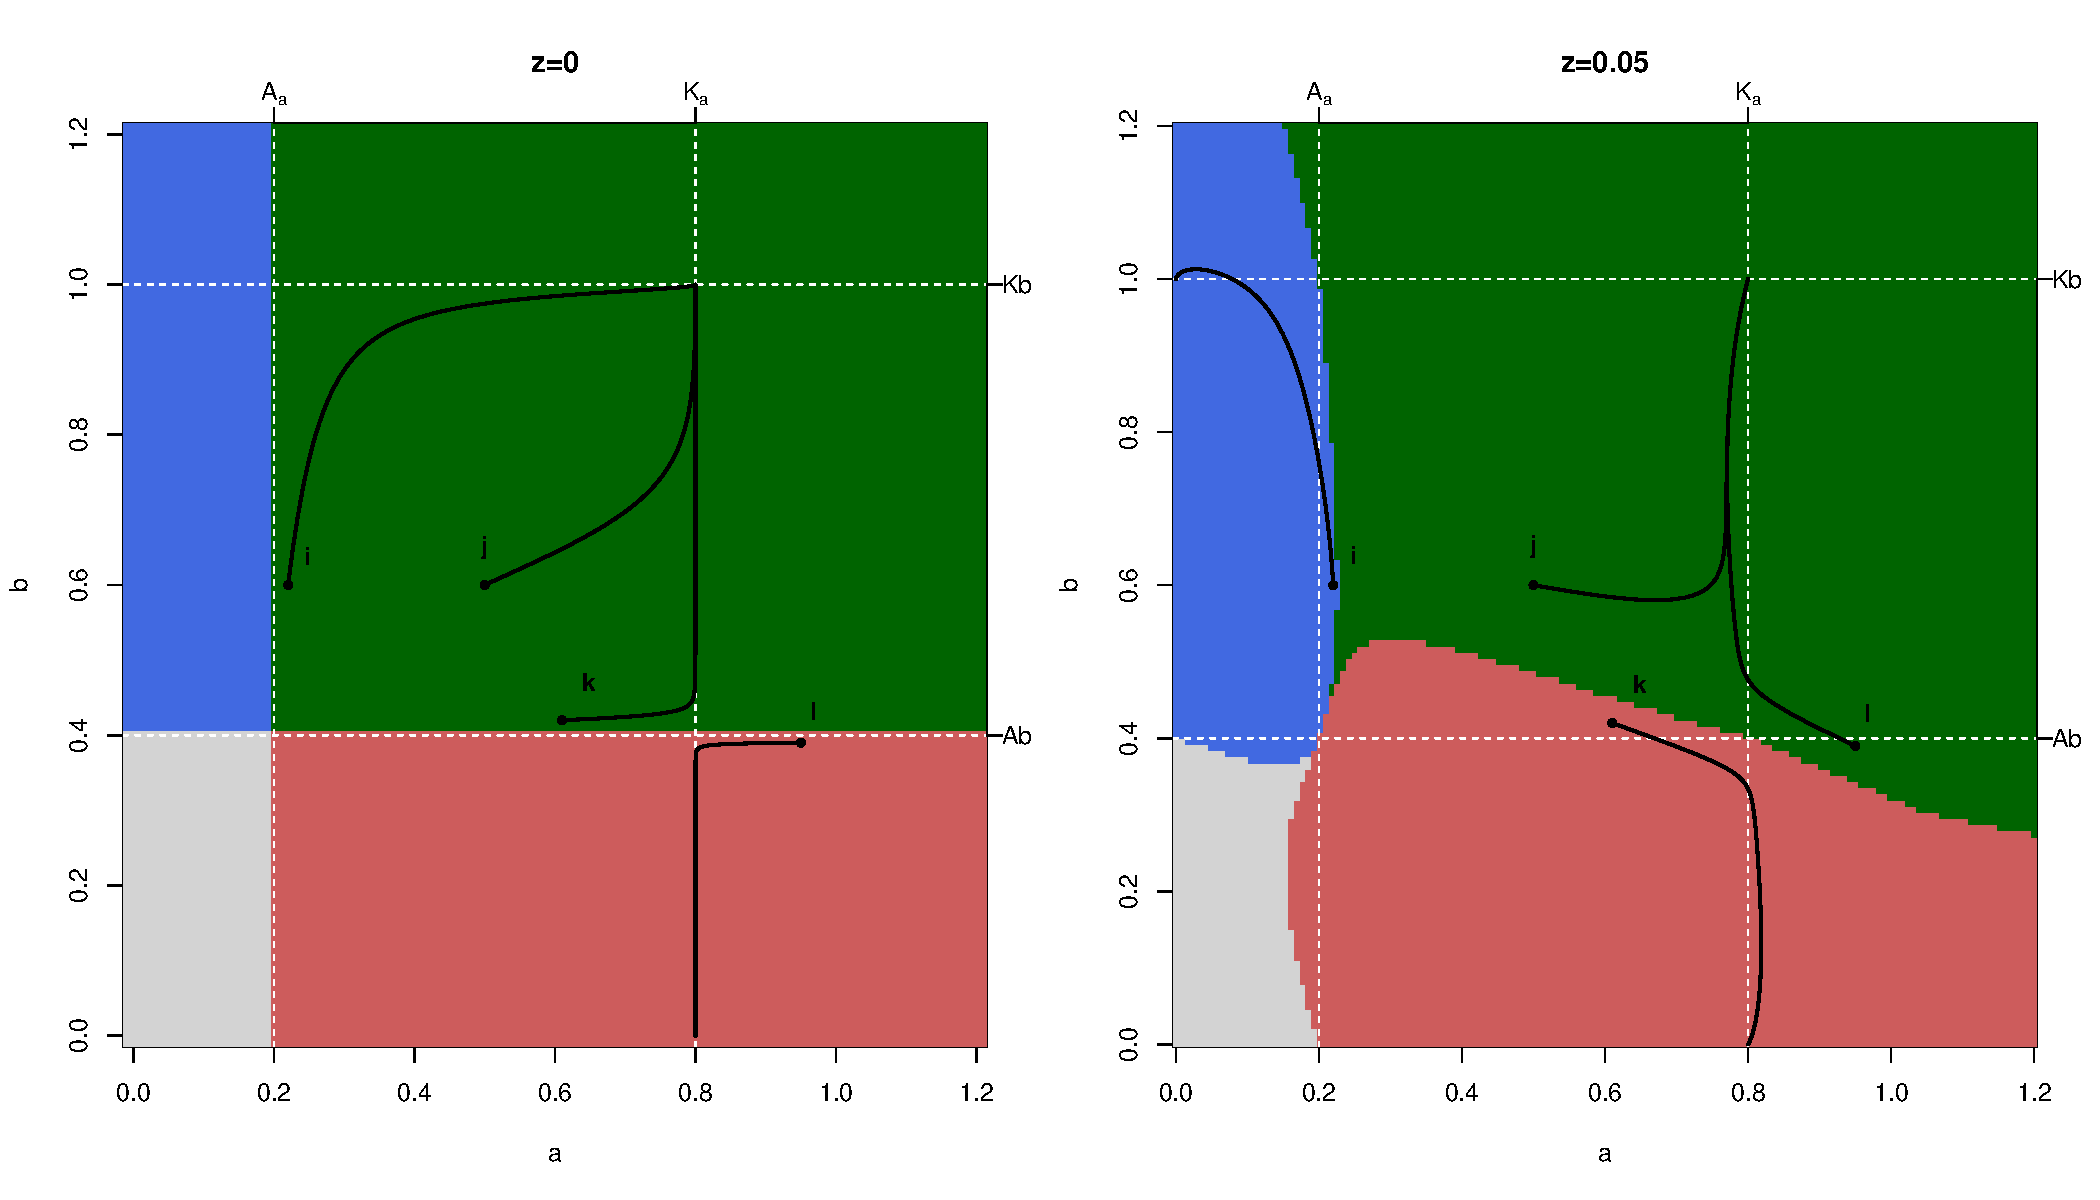
\includegraphics[width=\columnwidth]{./figures/figure3.pdf}
  \caption{Basins of attraction for the four equilibria (mutual extinction: grey; extinction of $a$: blue; extinction of $b$: red; stable coexistence: green) with (right) and without (left) social learning. Model parameters: $A_a=0.2$; $K_a=0.8$; $A_b=0.35$; $K_b=0.95$; $r_a=0.05$; $z=0$ (left panel) and $z=0.2$ (right panel) }
    \label{fig:TransmissionBasin}
\end{figure*}

Second, when the magnitude of social learning is high, the system is subject to effects similar to those observed with an increase in the per capita growth rate $r$ (cf. fig. \ref{fig:bifurcationDiagram}), that is a decrease in the stability of the fixed points. Figure XXXX shows an example where the increase in $z$ generates a transition from stable coexistence to cyclical fluctuations. %We need to make this figure as time-series, or actually use the bifurcation diagram.  
This regime is prone to occur when both variants are initialised with high densities. %This refers to the basin plot figureUnstable1.pdf that you've already made. Given the description below, do you think that those tiny "islands" of orange inside the green are actually specific values that are covered by the fluctuations in the time-series? Given that the system is deterministic, it wouldn't be a surprise, if anything there MUST be a combination of values for these... 
In these conditions the total density is too high to ensure a stable coexistence, and the regulatory effect of negative fitness is minimised by the fast rates of cultural transmission (i.e. individual shift strategy before experiencing a population decline resulting from density being over $K$). Figure XXX2 also implies that high reliance on social learning leeds to the emergence of a new basin of attraction for these unstably cycles, with small differences in initial conditions leading again to profoundly different dynamics. 


%\begin{figure}
%  \centering
%      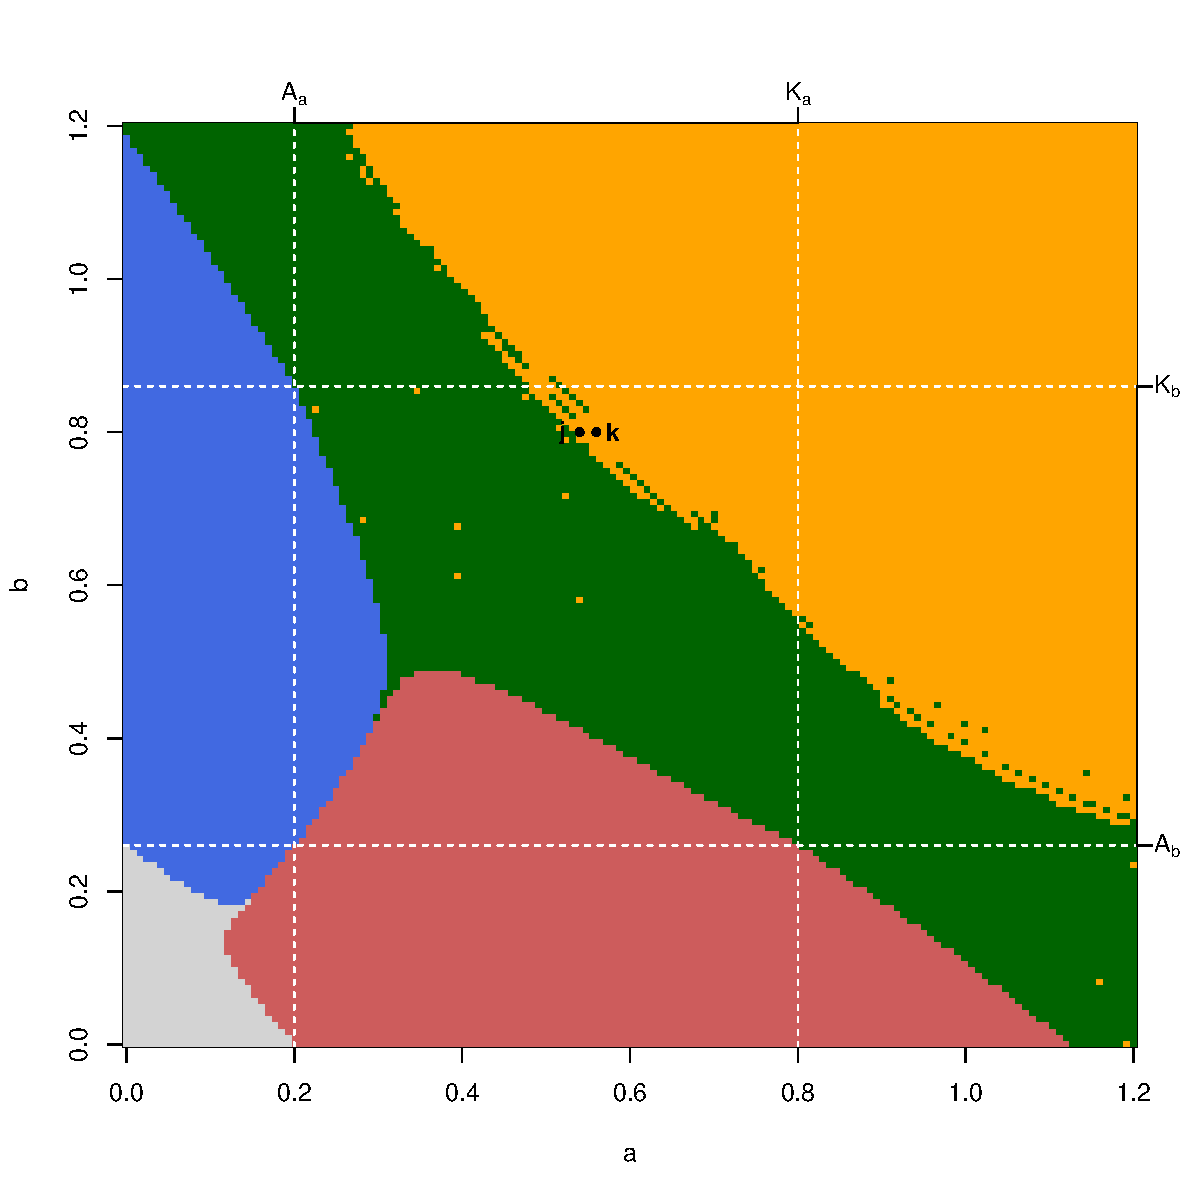
\includegraphics[width=0.5\textwidth]{./figures/figureUnstable1.pdf}
%  \caption{}
%    \label{}
%\end{figure}

%\begin{figure}
%  \centering
%      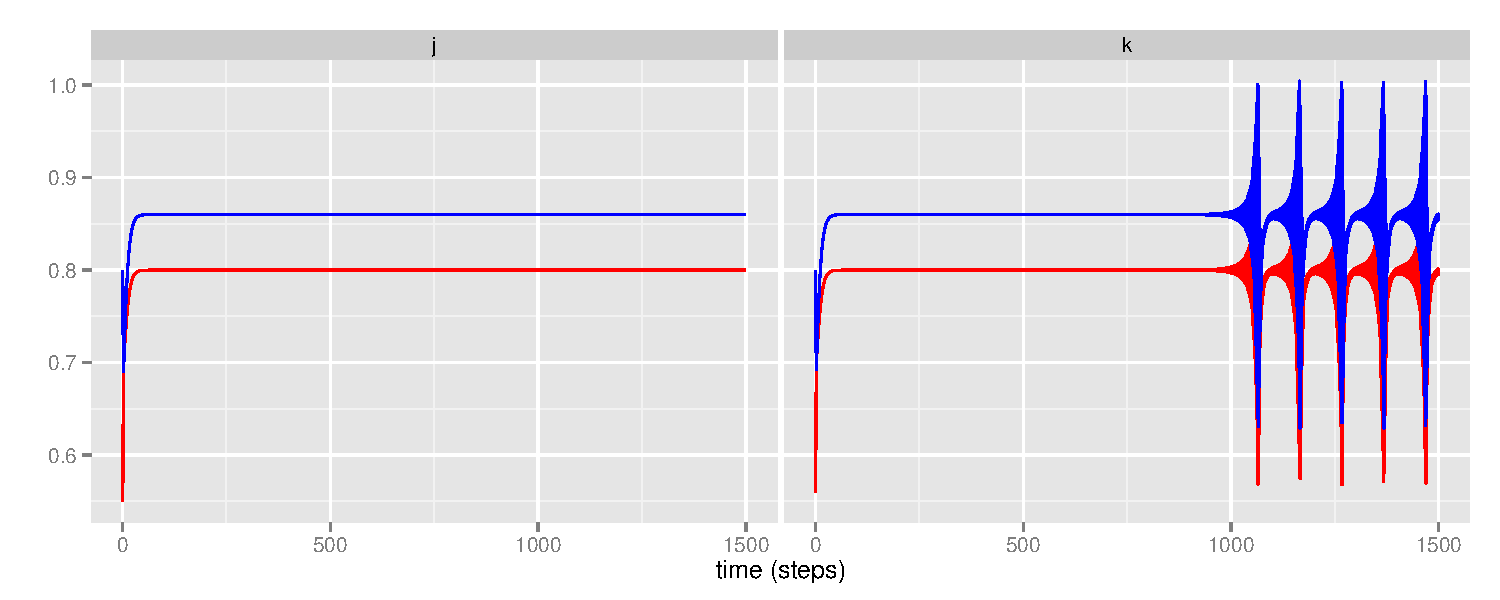
\includegraphics[width=0.5\textwidth]{./figures/figureUnstable2.pdf}
%  \caption{}
%    \label{}
%\end{figure}

\subsection{Differences in critical density and carrying capacities}

The analyses of the previous section suggest that maximum proportion of population that can switch strategies (i.e. the $z$ parameter) has major effects on the final equilibria (c.f. fig. XXX?). However, this will also depend on the key parameters defining the range of positive payoff for the two strategies (i.e. $[A_a,K_a]$ and $[A_b,K_b]$). While a comprehensive analysis is not possible, here we illustrate the relationship between these parameters and $z$ by introducing a new parameter $\lambda \in (0,1)$ adding the following constraints to equation \eqref{eq1}: 

\begin{equation}
\begin{aligned}
\label{eqOverlap}
A_b = A_a + (1-\lambda)(K_a-A_a)\\
K_b = K_a + (1-\lambda)(K_a-A_a)
\end{aligned}
\end{equation}

Equation \eqref{eqOverlap} ensures that the difference between carrying capacity and critical density is hold constant and equal between the two variants, so that $\lambda$ can be interpreted as an inverse  measure of overlap. Indeed when $\lambda=1$ the two variants are identical, and when $\lambda=0$, the critical density of one strategy becomes equal to the carrying capacity of the other (i.e. $A_b=K_a$). Figure \ref{fig:overlap} examines three different settings of $\lambda$  with low ($z=0.05$) and intermediate ($z=0.2$) degree of reliance on social learning. The plot suggests that, higher values of $z$ limits the number of initial conditions within the positive payoff zone (i.e. when the initial conditions for $a$ and $b$ are within the intervals $[A_a,K_a]$ and $[A_b,K_b]$) where a stable co-existence is achieved, but the magnitude of this effect is smaller for lower values of $\lambda$ (i.e. smaller overlap). We can further investigate this point by computing the relative areas of different basins of attraction within the positive payoff ozone for different parameter combinations of $z$ and $\lambda$. The results (fig. \ref{fig:percentages}) confirms that indeed with high overlap and high rates of social learning conditions enabling the stable coexistence is reduced, initially as an increase of conditions promoting the dominance of one variant or another, and eventually as the unstable fluctuations regime take over. With decreasing $\lambda$ unstable regimes vanish, and the relationship between $z$ and the size of the basin of attraction for stable coexistence becomes more or less constant for each value of $\lambda$. 

\begin{figure*}
  \centering
      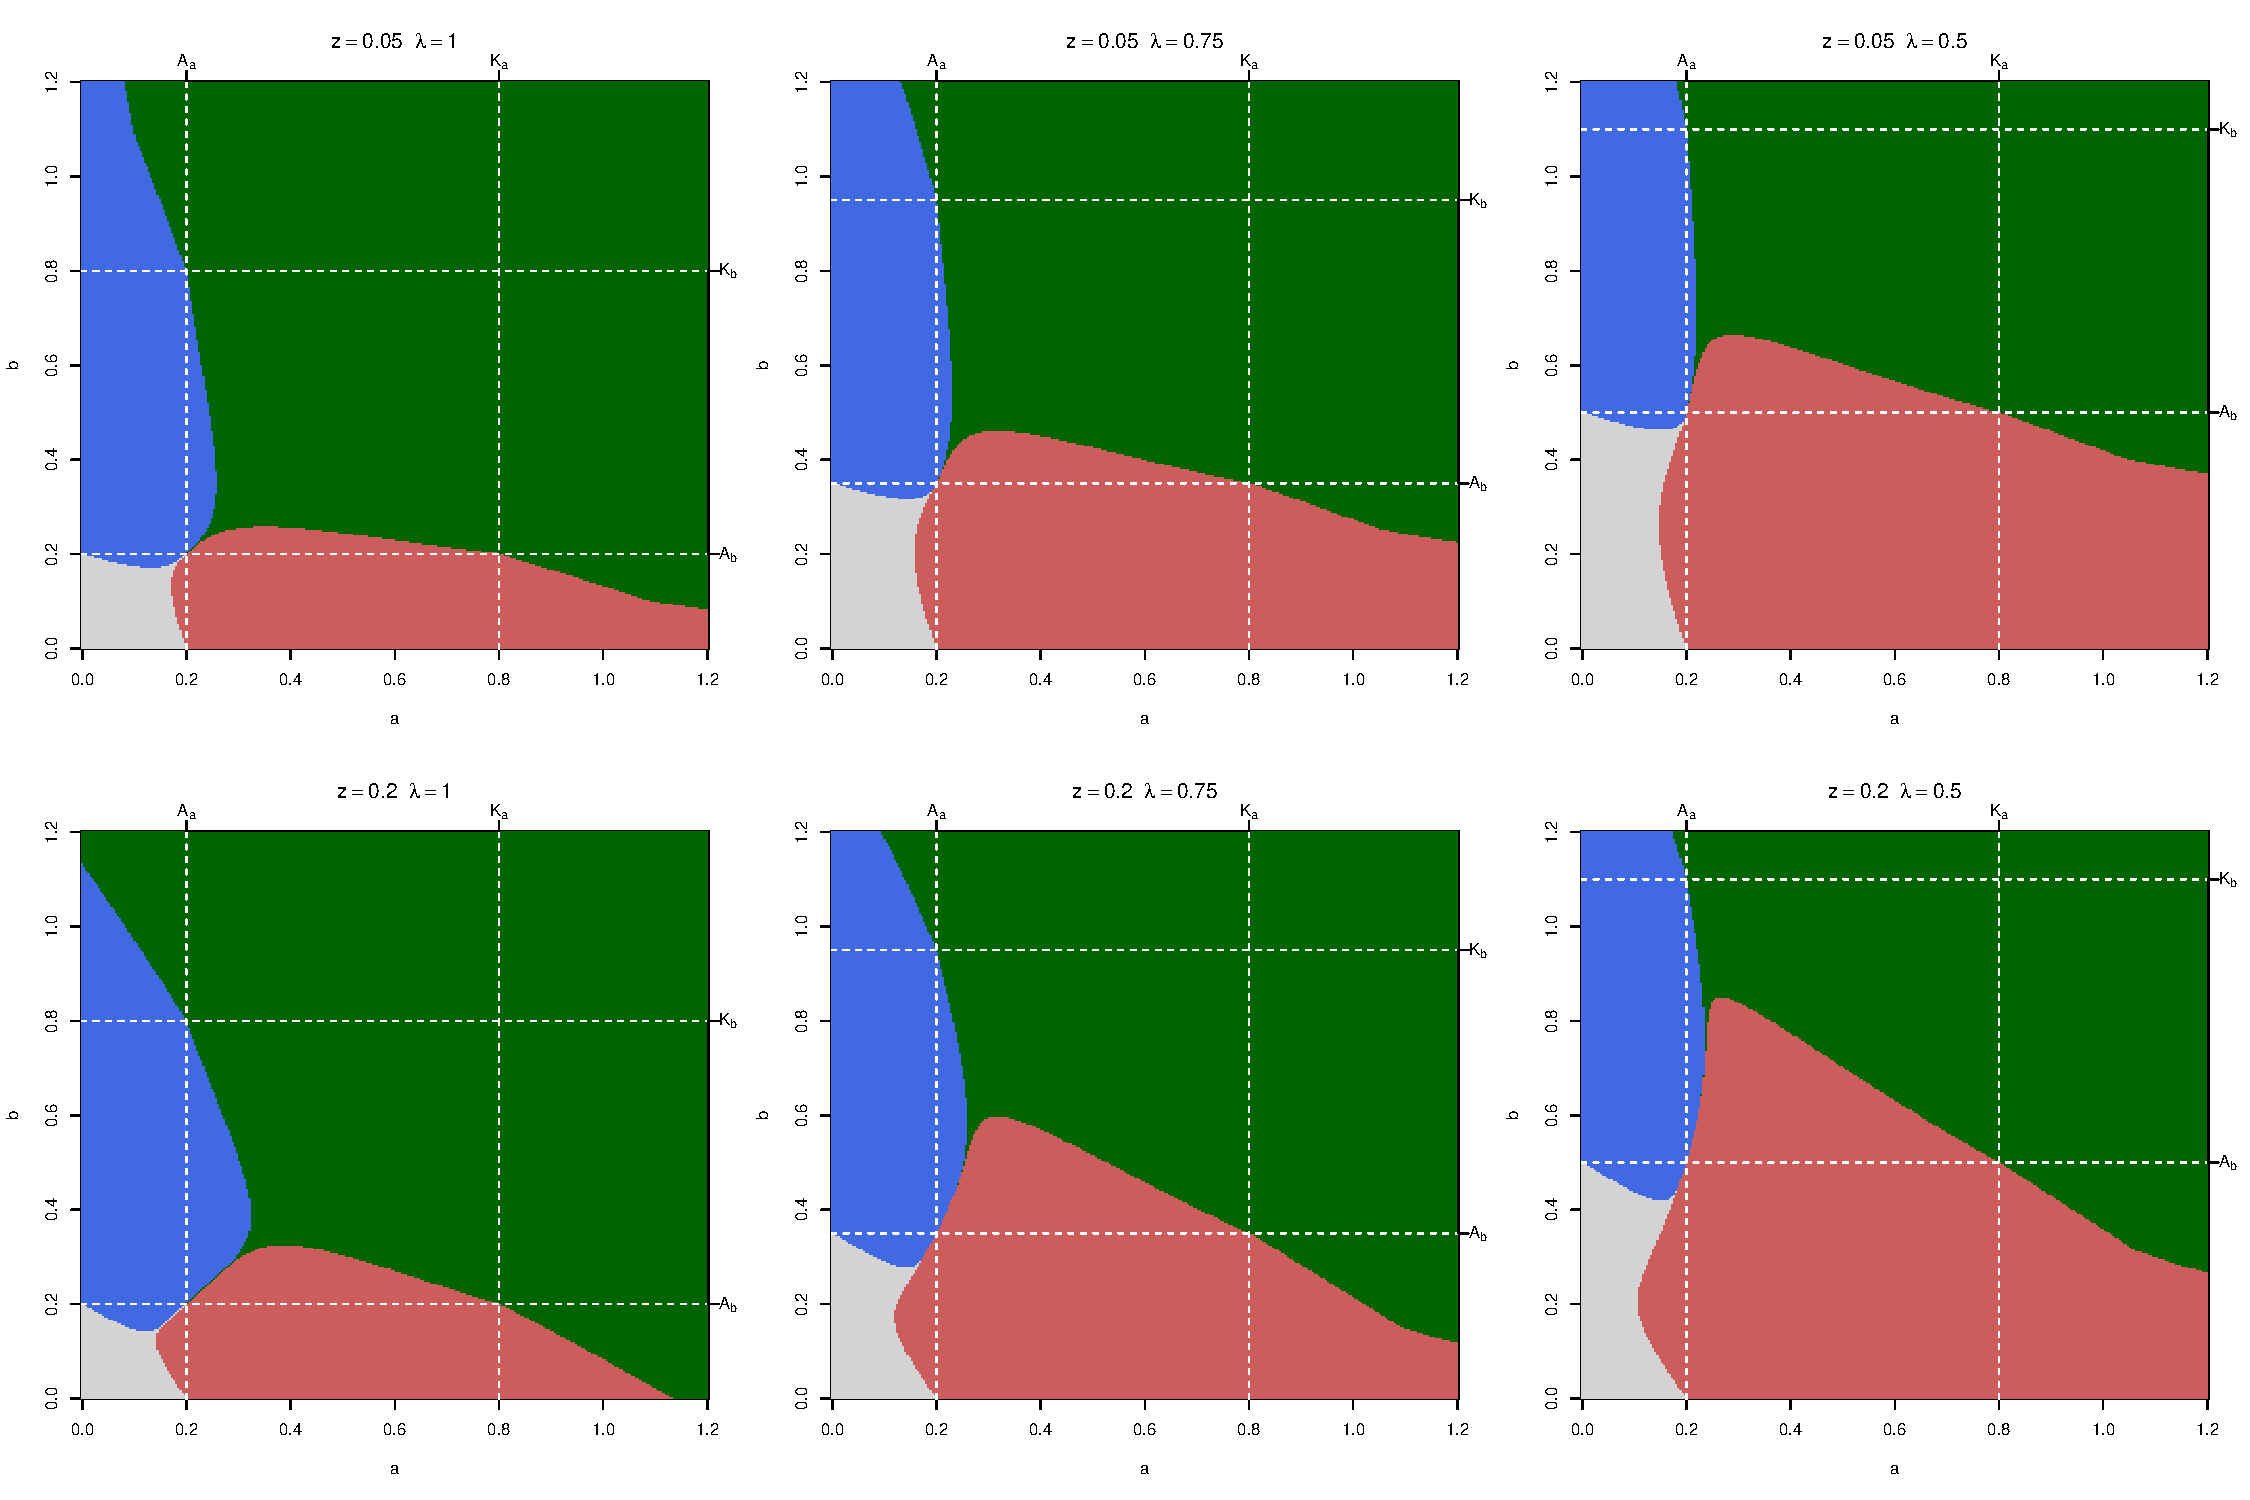
\includegraphics[width=\textwidth]{./figures/figure5}
  \caption{Basins of attraction for $z=0.05$ (top) and $z=0.2$ (bottom); $\lambda=1$ (left), $\lambda=0.75$ (middle) and $\lambda=0.5$}
    \label{fig:overlap}
\end{figure*}

\begin{figure*}
  \centering
      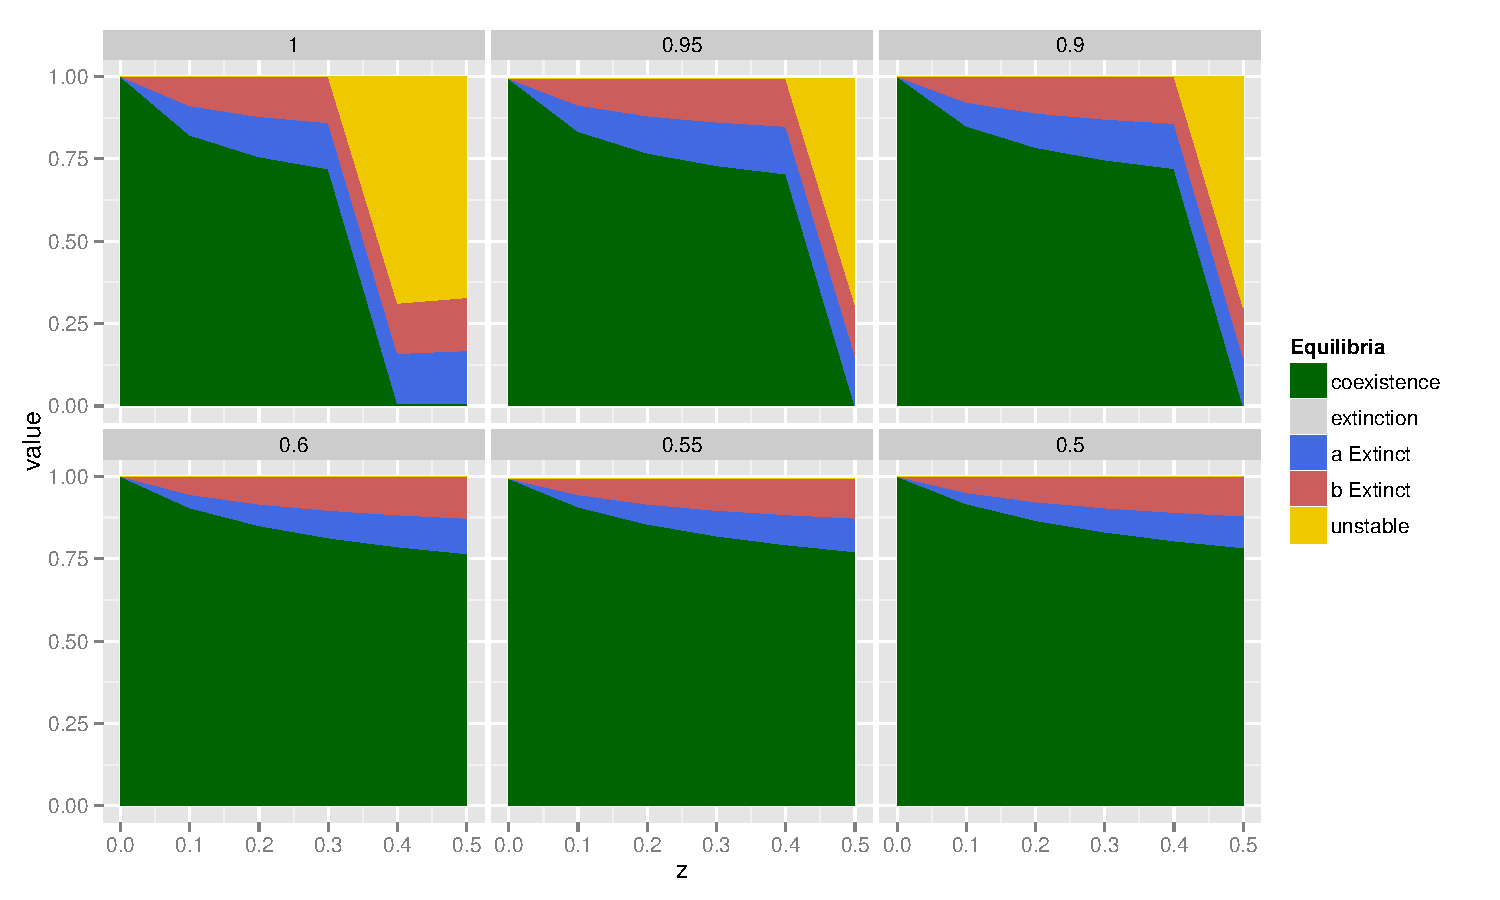
\includegraphics[width=\textwidth]{./figures/figure6}
  \caption{Proportion of initial conditions falling in each basin of attraction for different values of $\lambda$. X axis controls the parameter $z$ defining social learning. Model parameters: $A_a=0.2$; $K_a=0.8$; $r_a=0.05$}
    \label{fig:percentages}
\end{figure*}

\subsection{Effect of competition}

%This section needs to be revised:
Figure \ref{fig:percentages} also suggest that with decreasing values of $\lambda$, the variant with lower carrying capacity/critical density expands its basin of attraction. This implies that, with other things being equal, traits with higher $A$ and $K$ have a smaller number of favourable conditions that can promote its existence. Indeed in the case of the two-variants model examined here, the strategy with higher $A$ and $K$ can survive primarily when its initial density is comparatively high (e.g. above or equal its maximum payoff) and when the alternative strategy is close to its carrying capacity. The latter condition implies that novel strategies with higher carrying capacity but also higher critical densities are fully adopted only when the extant strategy with lower $A$ and $K$ has a density closer to its upper threshold. Thus innovations capable to sustain larger population density requires either a comparatively lower critical density that ensures a higher overlap with extant strategies, or an initial number of adoptees that are not guided by a payoff-based transmission. A third option, which we briefly explore here, is to relax the assumption that the payoff of each variant is exclusively a function of their intrinsic density. For instance several subsistence strategies do not have fully independent resource pools, and hence the success of a given variant might be detrimental to the payoff of the other irregardless of the effects provoked by cultural transmission. We can revise our core model by including new terms portraying the competition effect between the two resources:  

\begin{equation}
\begin{aligned}
R_{a,t}& = r_a (\frac{a_t-c_{A_a}b_t}{A_a}-1)(1-\frac{a_t-c_{K_a}b_t}{K_a})\\
R_{b,t}& = r_b (\frac{b_t-c_{A_b}a_t}{A_b}-1)(1-\frac{b_t-c_{K_b}a_t}{K_b}) 
\label{eqCompetition}
\end{aligned}
\end{equation}

where the four new parameters $c_{A_a}$, $c_{A_b}$, $c_{K_a}$ and $c_{K_b}$, measure respectively the negative (or positive) effect determined by the number of individuals of the “other” traits. When $c_{A}>0$ the Allee threshold is essentially increased, while when $c_{K}>0$ the carrying capacity is diminished as function of the other population. Larger values of any of the $c$ parameters dictates a stronger influence of the other population. 

%We need to mention that analytical equilibrium solution and put the equations here. Then discuss about the effects for different values of z. 



%what if competition
%show new stable points
%show dynamics? 


Figure \ref{fig:competition} shows a scenario where strategy $a$ is dominant over strategy $b$.

\begin{figure*}[h!]
  \centering
      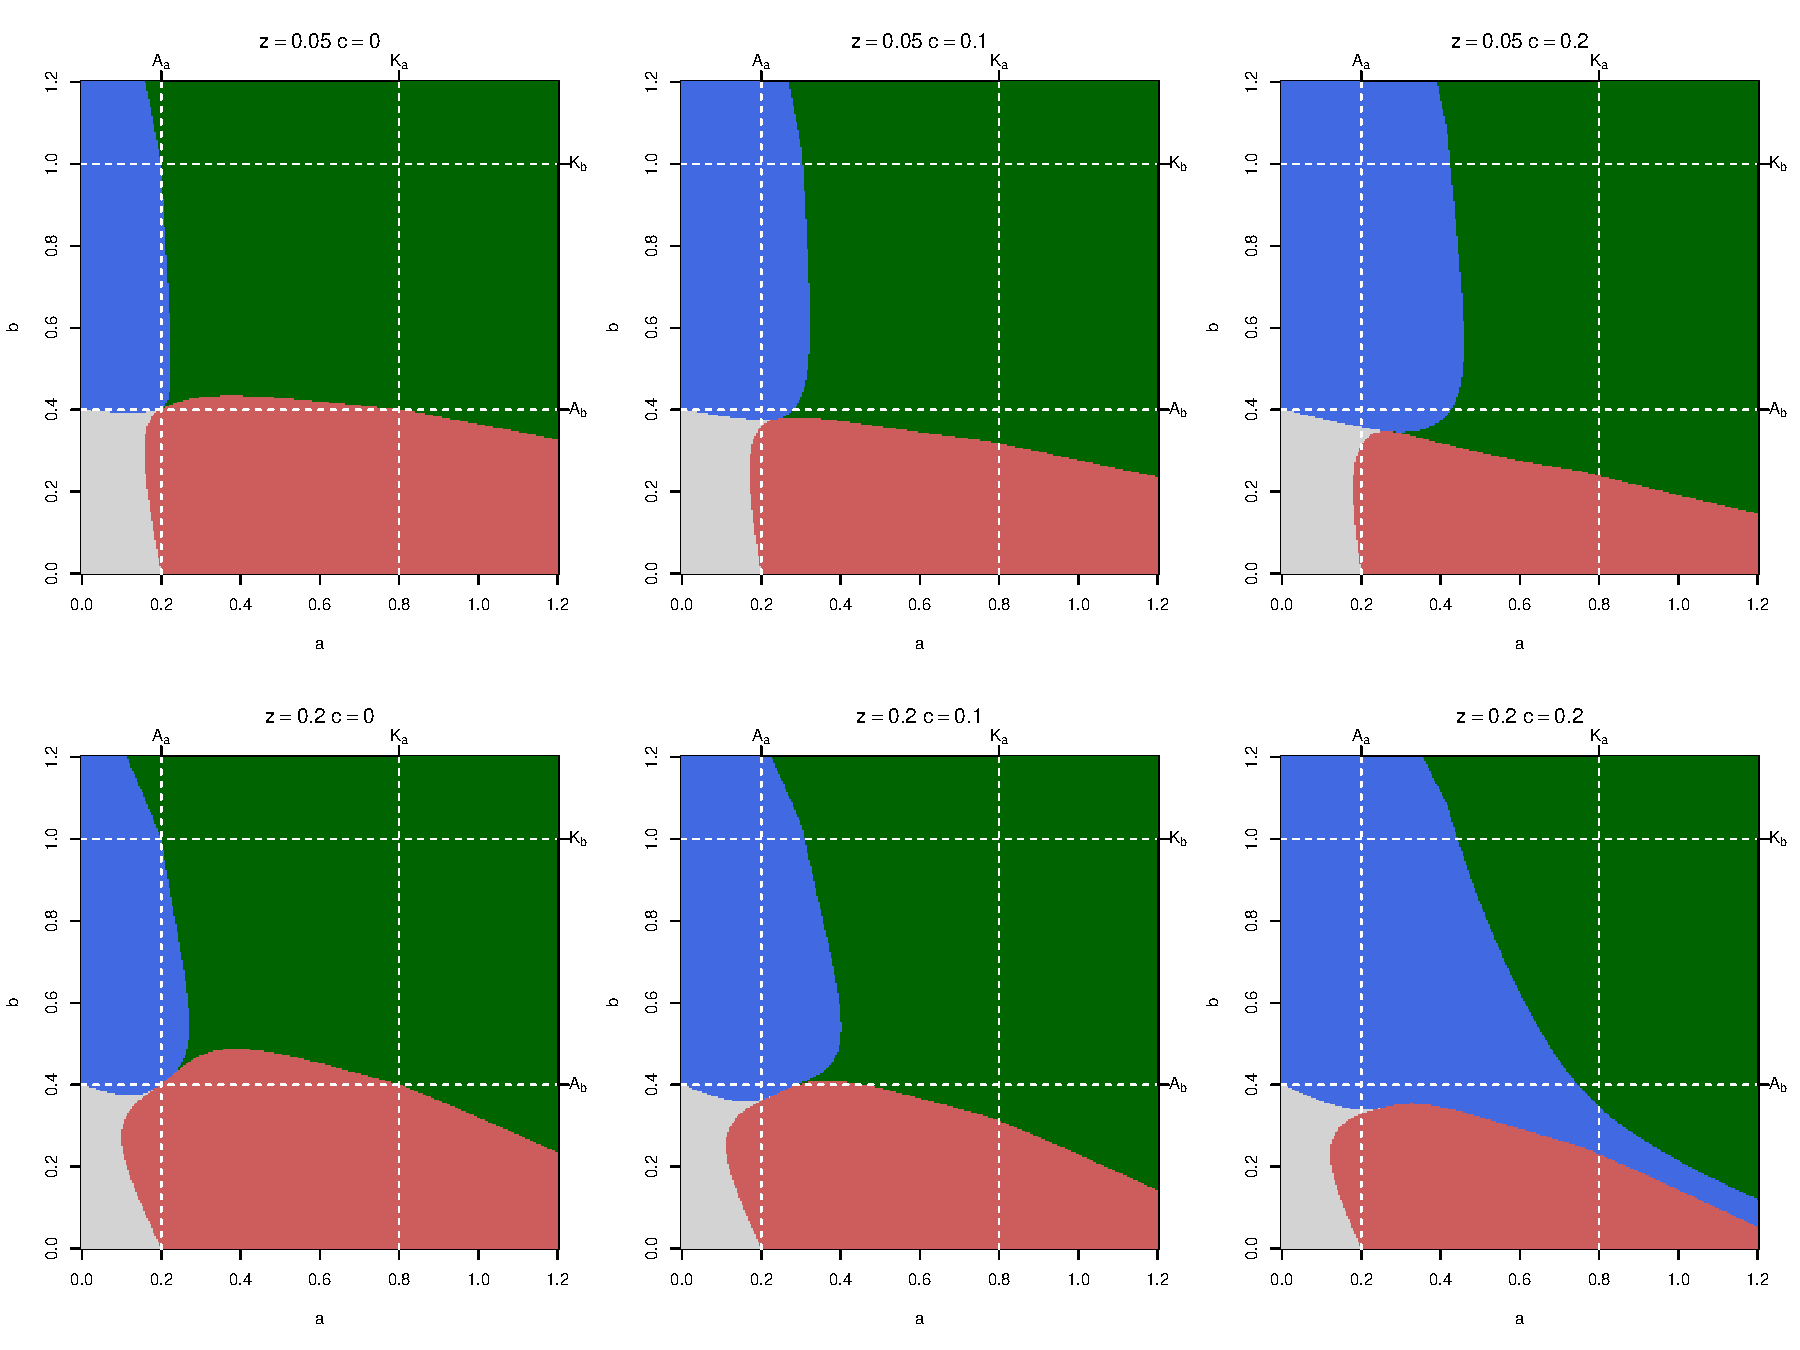
\includegraphics[width=\textwidth]{./figures/figure7}
  \caption{The impact of competition on the basins of attraction for the different equilibria. The Parameters used are $z=0.05$ (left) and $z=0.2$ (right) for social learning, and $c=-0.1$ (top) and $c=0.1$ (bottom) for competition.}
    \label{fig:competition}
\end{figure*}

% XAVI some brief discussion on results here, and update the dashed lines

% Do we need more? Perhaps another iteration of the overlap analysis with the competition promoting the variant with higher critical density and carrying capacity?

\section{Discussion}

% Cooperation / Facilitation / and Niche Construction review ? 


Our analysis examined the impact of payoff-based social learning strategies in the evolutionary dynamics of cultural traits with direct and inverse density dependence. The results showed that social learning can alter the basins of attraction of stable nodes, leading to different dynamics and equilibria from the very same initial conditions. When the reliance on social learning is comparatively high, and  the two variants have a substantial overlap in their range of positive payoff (i.e. they share similar critical densities and carrying capacities), we also observe the emergence of a chaotic behaviour where the system fluctuates without reaching a stable equilibria. Our results imply that evolutionary trajectories that are generally expected from a standard two population Allee models can exhibit unexpected outcomes. Variants below critical density can survive and a stable coexistence of strategies above this threshold is not necessarily guaranteed. The effects of social learning can also be observed in the trajectories of these evolutionary dynamics . Reversions to lower densities do not exclusively occur only when the variant is above its carrying capacity, and when the reliance on social learning is high these episodes becomes more frequent and extreme in its magnitude. 

%Not sure where to put competition, maybe the whole thing should be in the appendix?

The implications of our model can provide some insights in the evolutionary history of subsistence traits in human history. Many prime examples of keystone innovations are closely related to the introduction of new subsistence strategies that enabled a larger carrying capacity, often coupled with the cost of higher critical densities. The spread of behavioural traits such as the know-how of the domestication process~\citep{barker2006} the use of new subsistence tools~\citep{petraglia_population_2009} and processing techniques~\citep{molleson1993}, as well as the inclusion/exclusion and extensification/intensification of different prey species are just some of the most notable examples. Both ethnographic and archaeological evidence show many instances where these critical transitions where not smooth, often leading to the coexistence of alternative strategies as well as episodes of a return to a previously abandoned strategies. %PUT HERE LIST of EXAMPLES. 
While in most cases these are more anecdotal evidence than testable empirical cases, the insights of our models suggests that different levels of reliance on social learning could in fact profoundly drive the system into different trajectories.  These insights can possibly contribute to existing models of subsistence shifts proposed in human behavioural ecology\citep{smith1992,bird2006,kennett2006}, combining its core theoretical framework to the one developed by cultural evolution studies. 






\section{References}

\bibliographystyle{elsarticle-harv}
\bibliography{references}

\section{Appendix I}

-50,000 iterations
-floating point arithmetic



\end{document}

